\section{Data exploration}
\label{sec:data_exploration}

Fluorescent Neuronal Cells images are high-resolution RGB pictures of constant shape (1200 pixels height by 1600 pixels width) collected under fixed experimental conditions.
In terms of features, the data can be explored at two complementary levels. 
In fact, interesting insights can be retrieved by looking at the color and luminance information carried by pixels. Also, conducting analogous analyses on the ground-truth masks reveals

% In terms of data features, the most interesting aspects regard the color and luminance information, the counts distribution and the cells characteristics.
% In terms of data features, the most interesting aspects pertain the color and luminance information, the counts' distribution and characteristics of the cells.
The data can be explored at two complementary levels: pixels features and cells characteristics. 
On the one hand, interesting insights can be retrieved by looking at pixels' color and luminance information. Also, analogous analyses on the ground-truth masks reveal essential information about class-imbalance between signal and background.
On the other hand, examining object properties can highlight potential nuisances and suggest how to evaluate model performances.

\subsection{Salient features}
\label{sec:data_features}

% As far as the color, t
The picture appearance is dominated by two prevalent tints due to the intentional selection of a specific wavelength: a darker hue corresponding to areas whose light was filtered out and a yellow tone emitted by the fluorophore
(\cref{fig:dataset:empty,fig:artifacts:clumping}).
As a consequence, the only color channels to be populated are red and green, while blue is typically empty. 
An example of this effect is reported in \cref{fig:dataset:pixel_intensity}, where the average distribution of pixel intensity is illustrated.
\begin{figure}
    \centering
    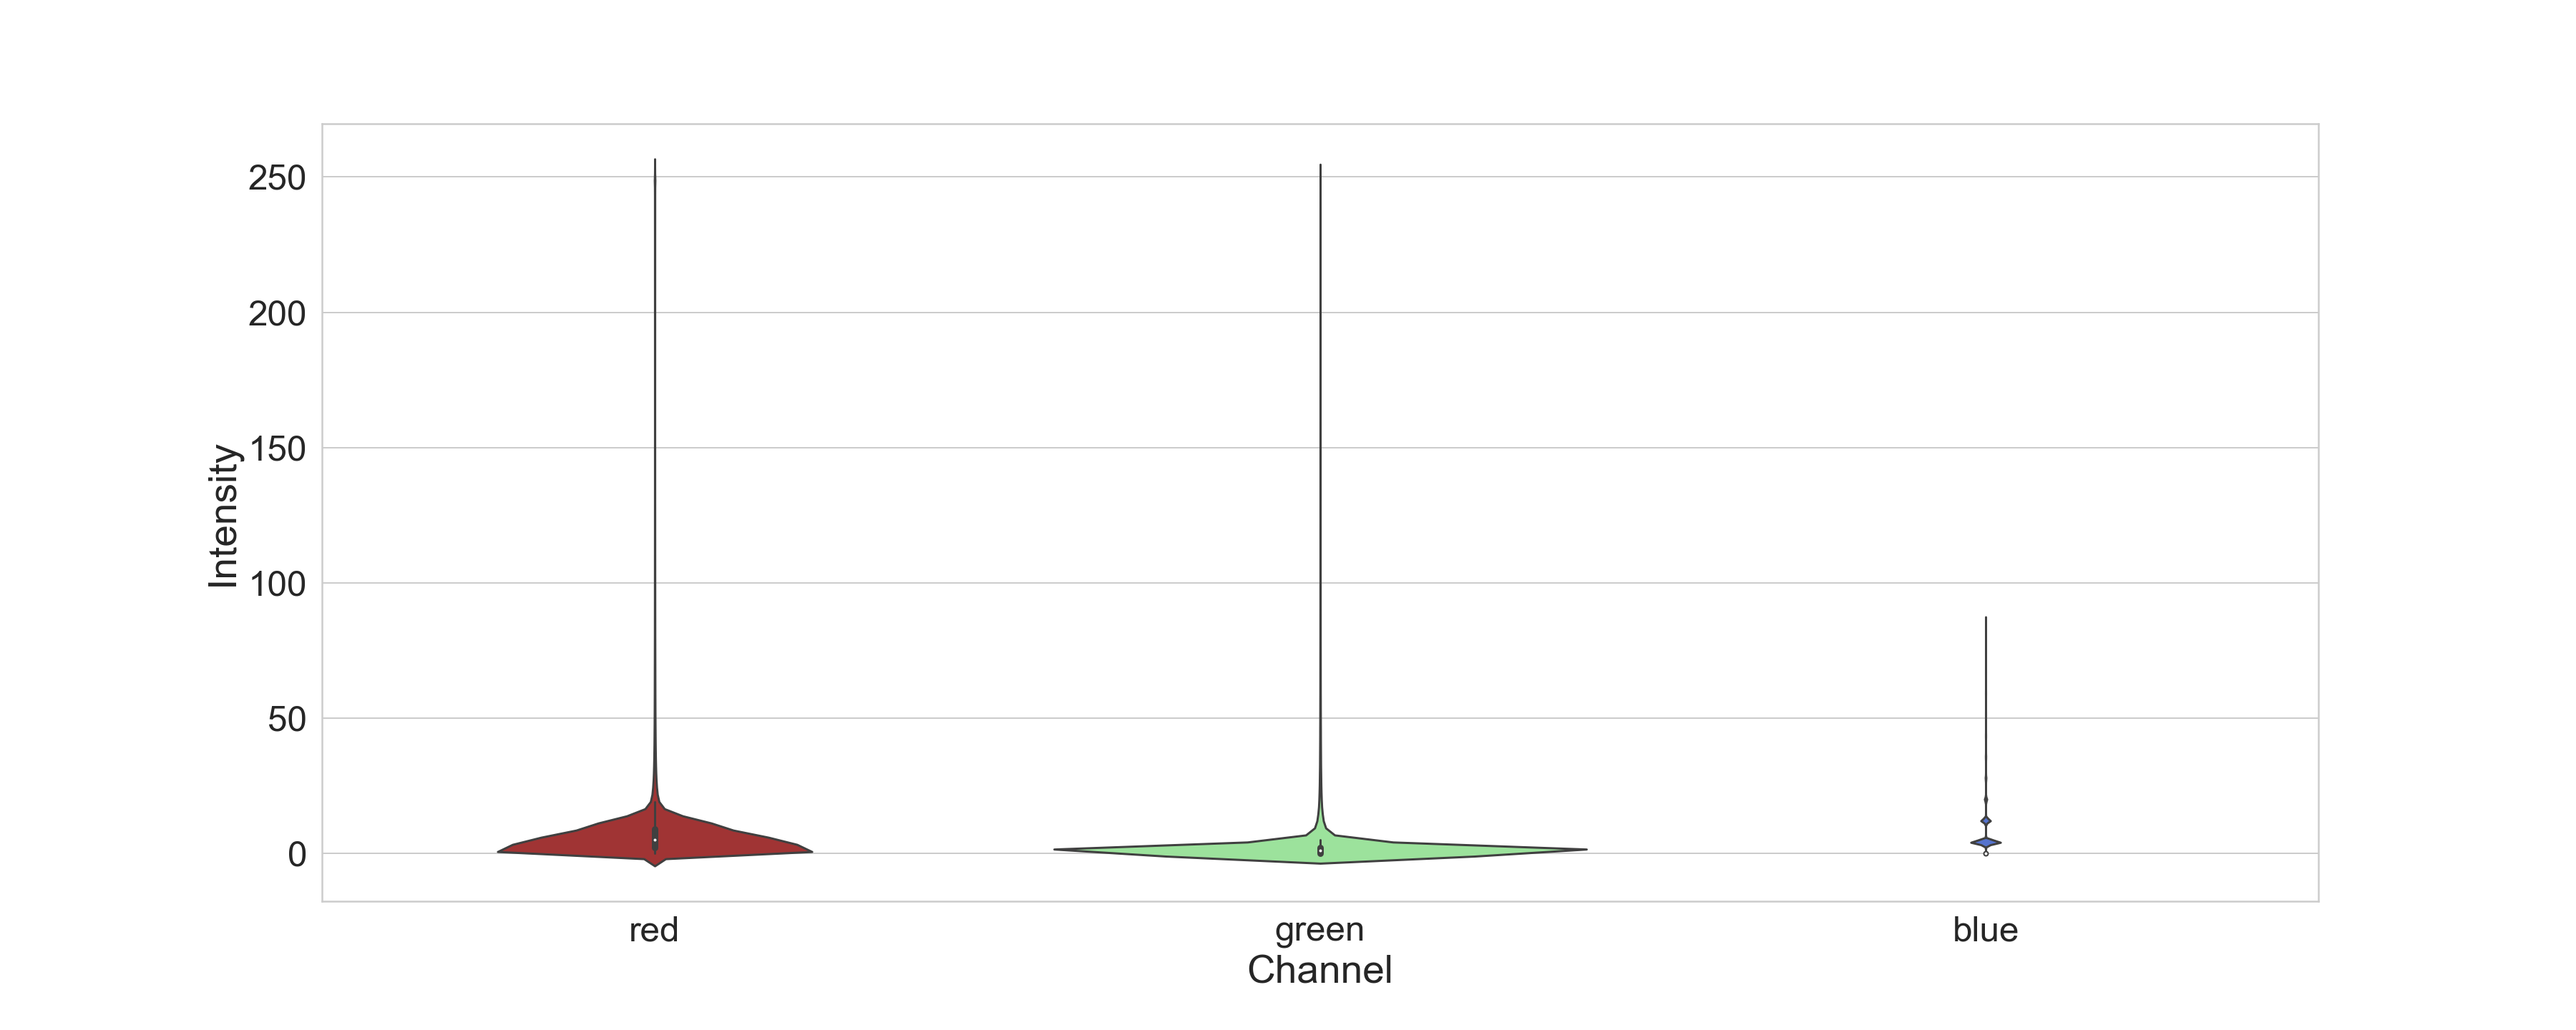
\includegraphics[width=\textwidth]{figures/120_dataset/pixel_intensity_distribution.png}
    \caption{Pixel intensity distribution. Violin plot of the average distribution of pixel intensities across the  RGB channels}
    \label{fig:dataset:pixel_intensity}
\end{figure}
Guided by this observation, one may argue that all this information is superfluous and resorting to a grayscale representation could be better since the images are ultimately shades of yellow.
\Cref{fig:dataset:colorspace} (left) corroborates this intuition, as most pixels lay almost on a straight line in the red-green plane. 
This suggests that the two channels are highly correlated, so a one-dimensional subspace may be enough to represent most of the variability of the data.
In turn, this would bring two advantages: ease the learning process -- as neural networks typically suffer when inputs are correlated %\cite{} 
-- and make it more efficient -- as one considers only one channel instead of three.

However, the use-case at hand has no stringent requirements in terms of computing resources and runtime, so the 3-channels training is still feasible.
More importantly, the information thrown away when converting to grayscale, although tiny, may still be crucial to discriminate background and signal. 
At the same, the RGB colorspace may not be the optimal representation to learn this separation. For instance, \cref{fig:dataset:colorspace} (right) shows the same images according to a different encoding, HSV. 
In this case, the separation between dark and colored tones appears more evident. 
Moreover, most of the pixels are concentrated in low hue values
and their distribution seems more spread across the saturation-value plane. 

All that being considered, this work tried to leverage the insights of both approaches. 
On one side, the RGB colorspace was taken as a starting point to exploit all available information. On the other, the model first layer was designed to incorporate a colorspace transformation from RGB to a single channel.
% In this way, the intent is to avoid introducing any colorspace-related bias by letting the model learn the most convenient representation and, at the same time, benefit from the computational advantage due to a lower dimensionality.
The intent is to avoid introducing any colorspace-related bias by letting the model learn the most convenient representation without ignoring the fact that a one-dimensional manifold is probably enough to express the variability of the data.
\begin{figure}
    \centering
    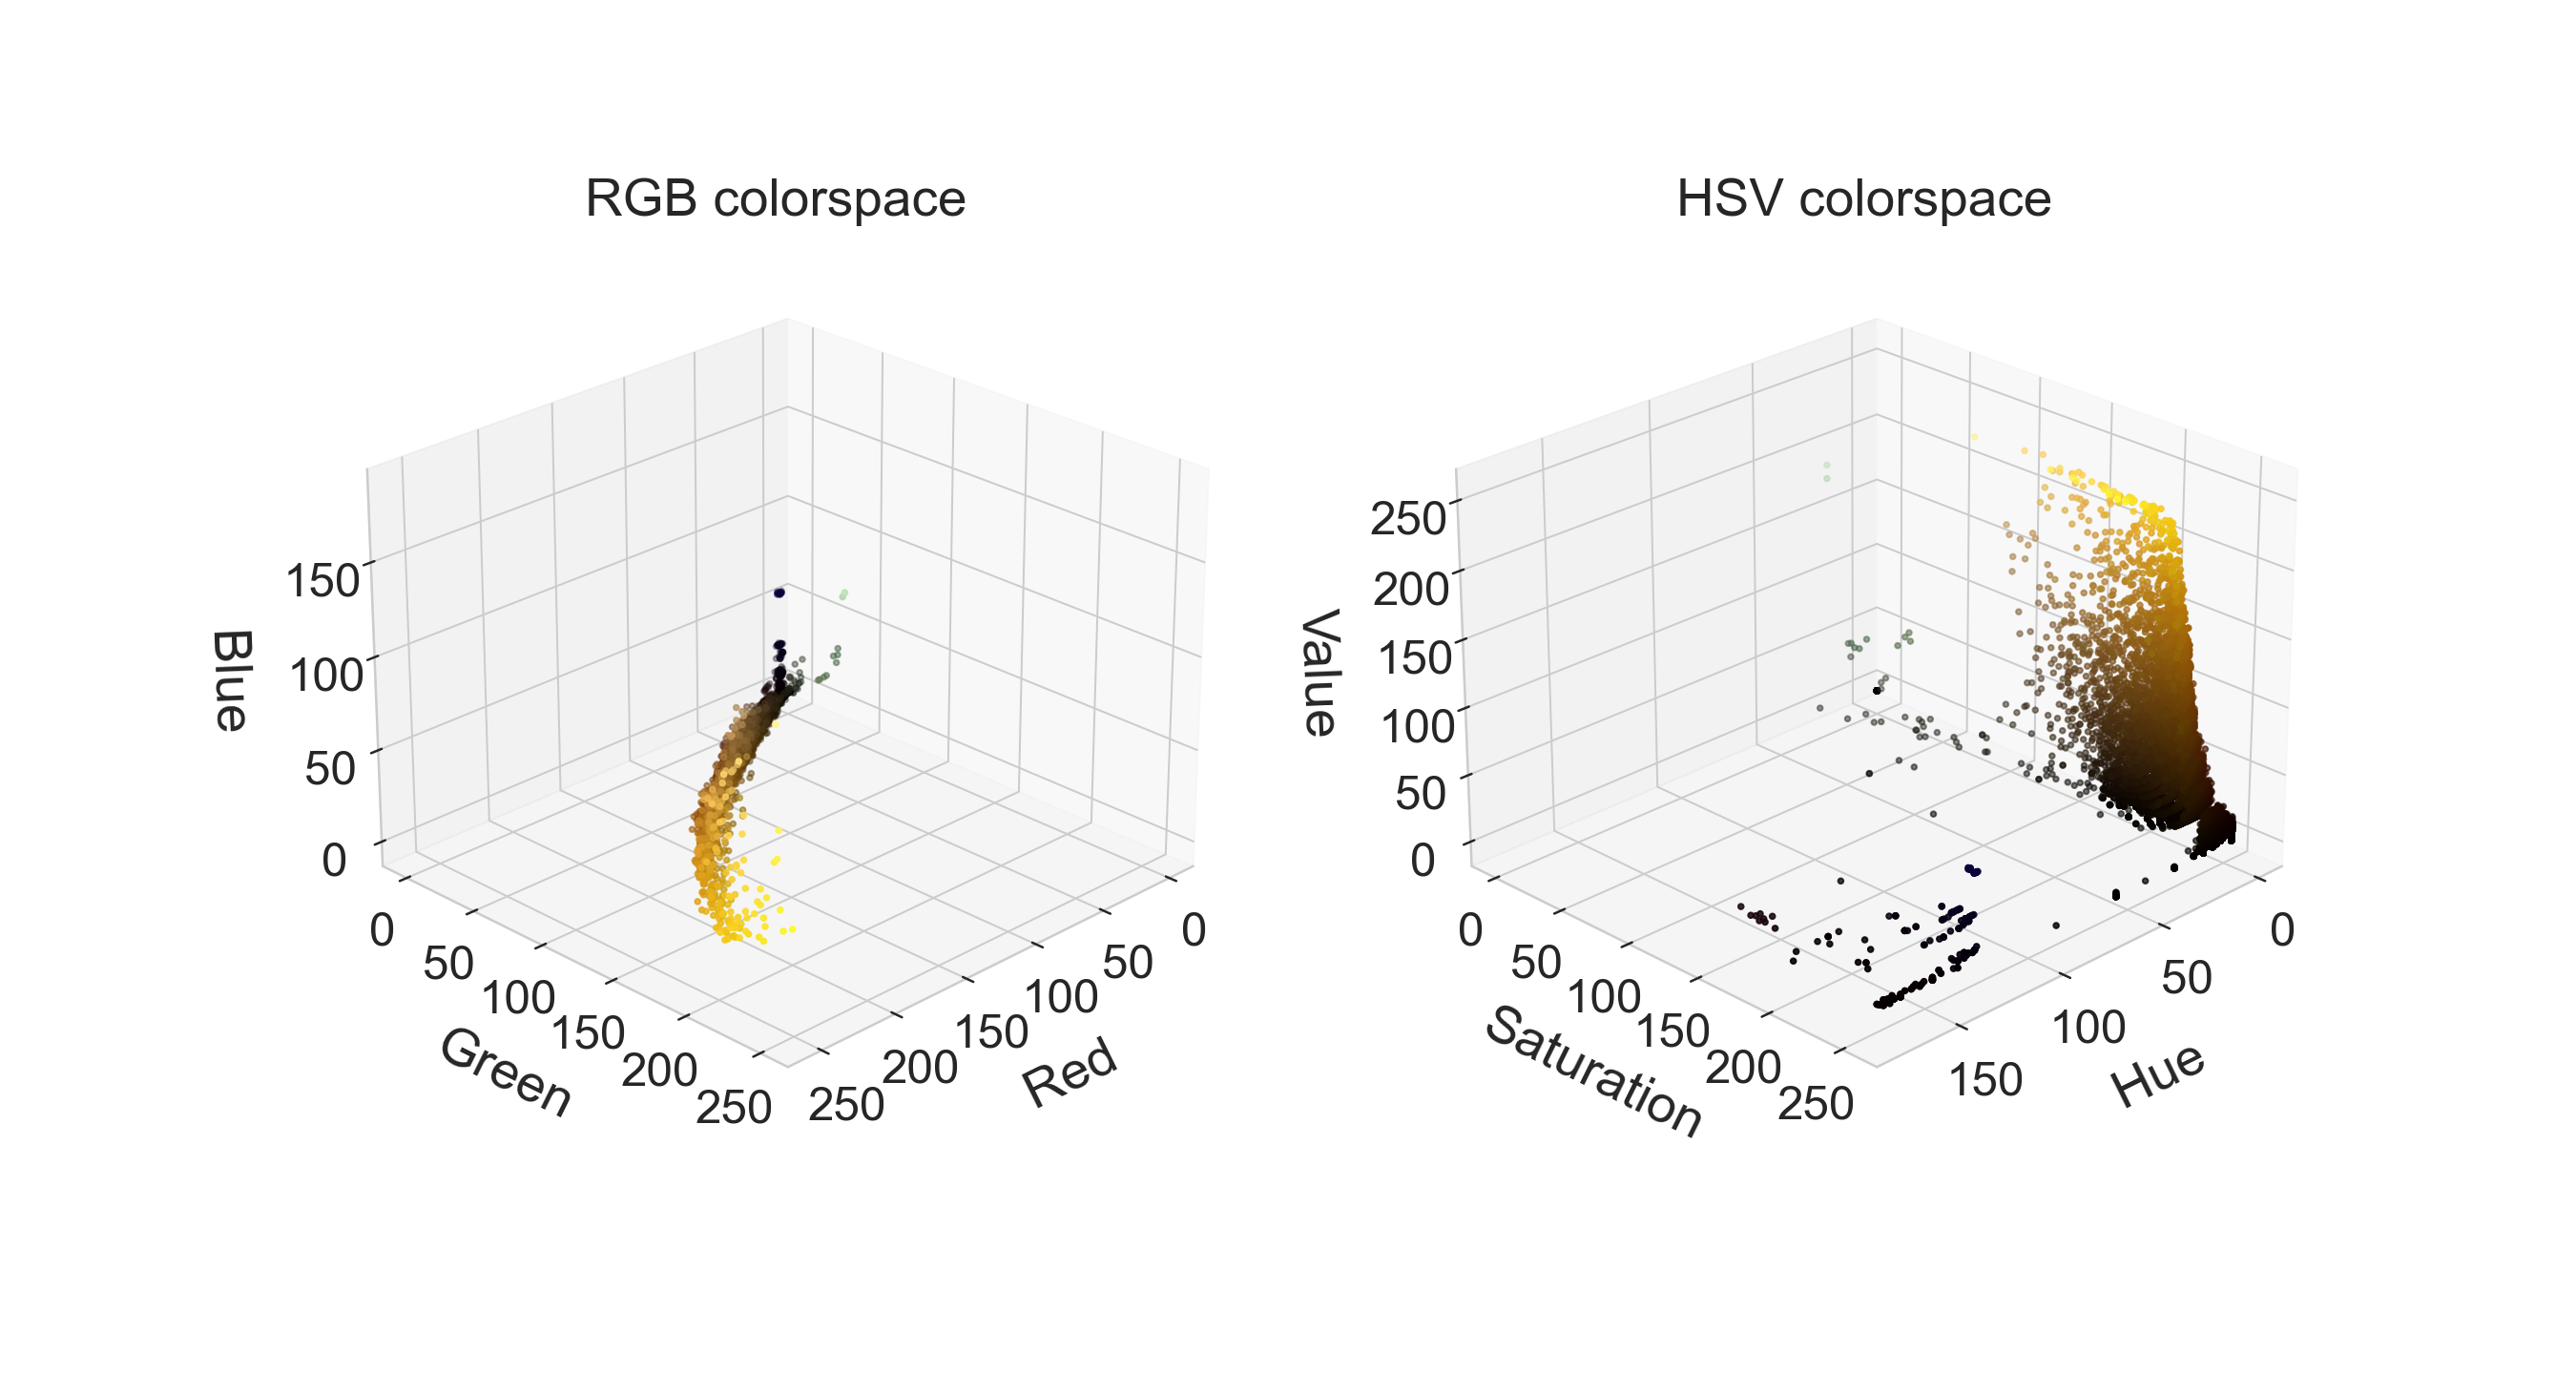
\includegraphics[width=1.1\textwidth]{figures/120_dataset/colorspace_Mar23bS1C2R3_VLPAGl_200x_y.png}
    
    \centering
    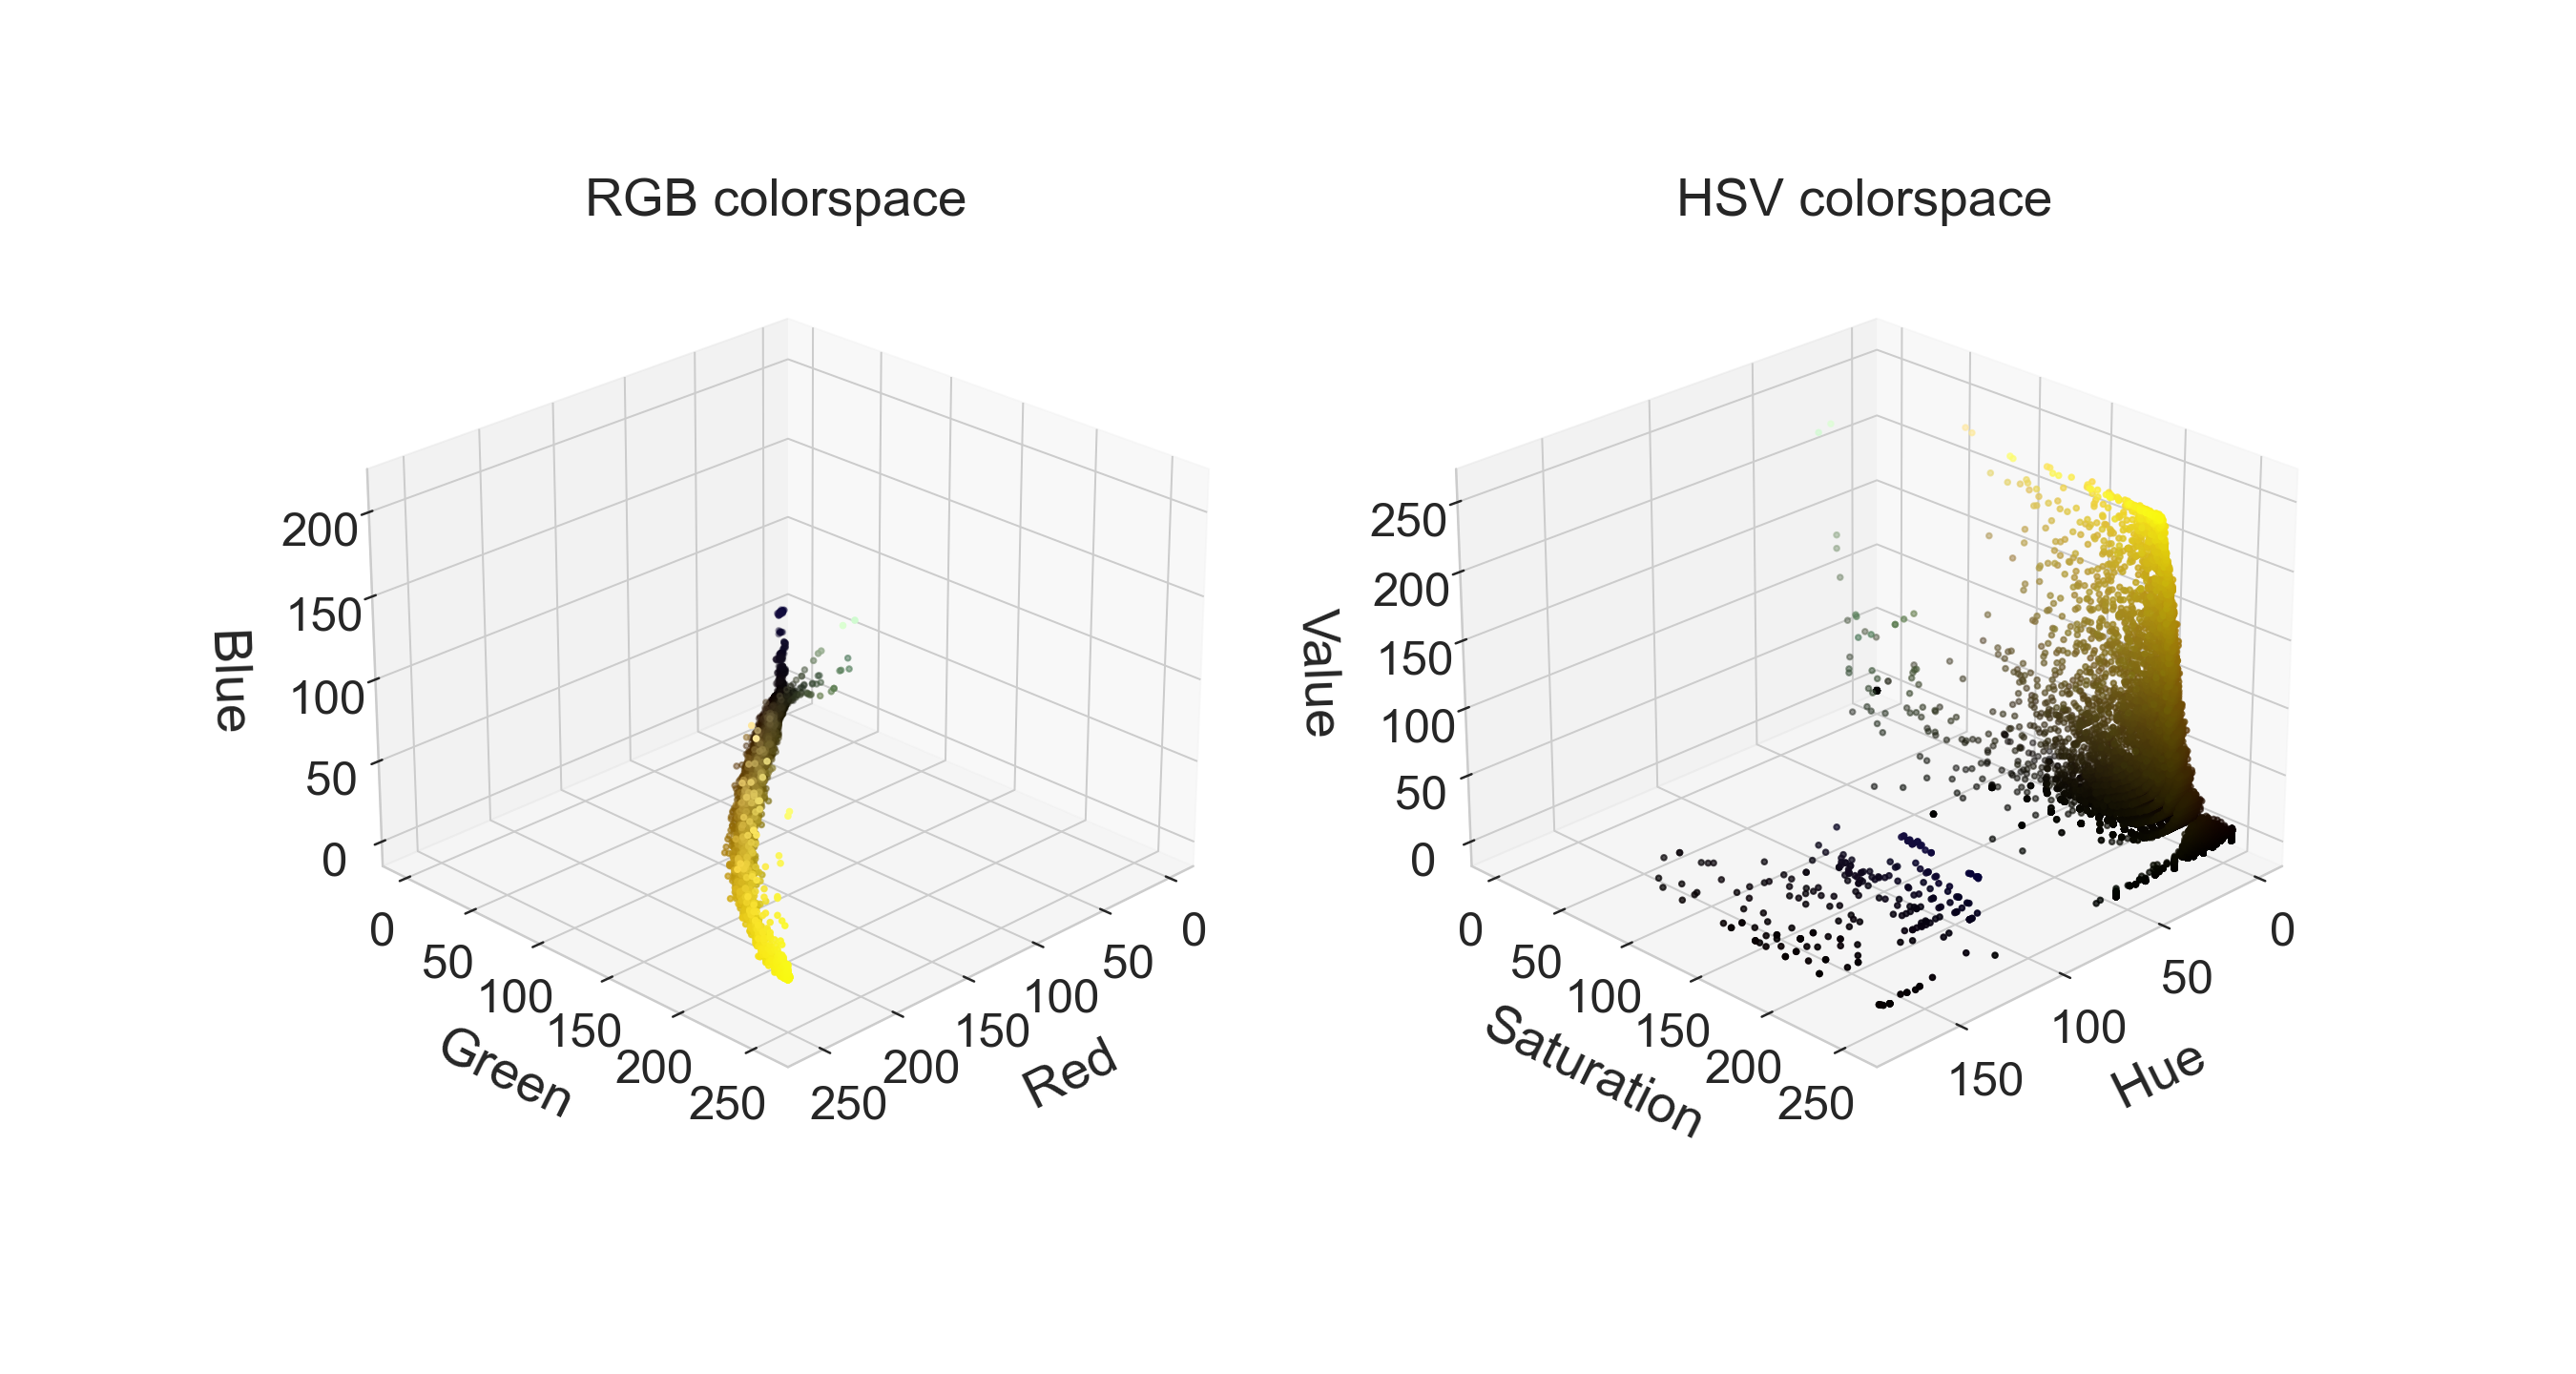
\includegraphics[width=1.1\textwidth]{figures/120_dataset/colorspace_Mar26bS2C1R2_DMl_200x_y.png}
    \caption{Colorspace representation. The same image is represented as RGB (left) and HSV (right). Pixels are treated as 3D points with coordinates given by their encoding in the corresponding colorspace}
    \label{fig:dataset:colorspace}
\end{figure}

\subsection{Class imbalance}
\label{sec:class_imbalance}
\begin{figure}
    \centering
    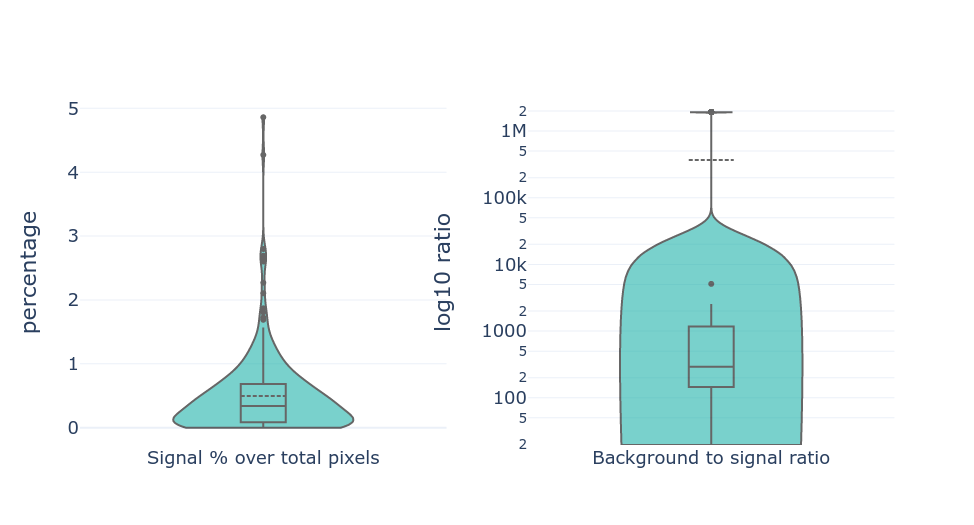
\includegraphics[width=\textwidth]{figures/120_dataset/class_imbalance.png}
    \caption{\textbf{Class imbalance.} Violin plot and boxplot of signal percentage (left) and background to signal ration (right).}
    \label{fig:dataset:class_imbalance}
\end{figure}

Inspecting ground-truth masks at pixel level reveals important characteristics that affect the training process. 
By looking at the cardinality of pixels belonging to the background and the signal it is possible to notice how the two classes are extremely unbalanced.
\Cref{fig:dataset:class_imbalance}) (left) shows the violin plot of the percentage of signal pixel over the total image pixels across the 283 pictures.
The distribution is deeply skewed towards 0, with a median of 0.34\% and a 90\emph{-th} percentile of 1.07\%. 
Hence, almost 90\% of the images contain less than 1\% of pixels belonging to the signal%
% , causing an extreme unbalance between signal and background classes
.
Even more significantly, the right tail does not exceed 5\% of signal coverage, with a maximum of 4.86\%.

\Cref{fig:dataset:class_imbalance}) (right) illustrates the same concept but focuses on the relative proportion of background to signal. 
The distribution is left-skewed, with a lower half concentrated in the range (19, 291), i.e. background pixels are roughly from 20 to 300 times the signal pixels in 50\% of the images.
Remarkably, the disproportion grows even faster in the right tail, where the ratio explodes up to over 1000. 
Finally, notice that the bulk of outliers accumulates in the higher end of the domain. 
This is caused by the contribution of empty masks that cover more than 10\% of the total images.


These considerations imply that dedicated training strategies are needed for the model to face this strong class imbalance and correctly learn to classify image pixels.

\subsection{Objects features}
\begin{figure}
    \centering
    \subfloat[Area]{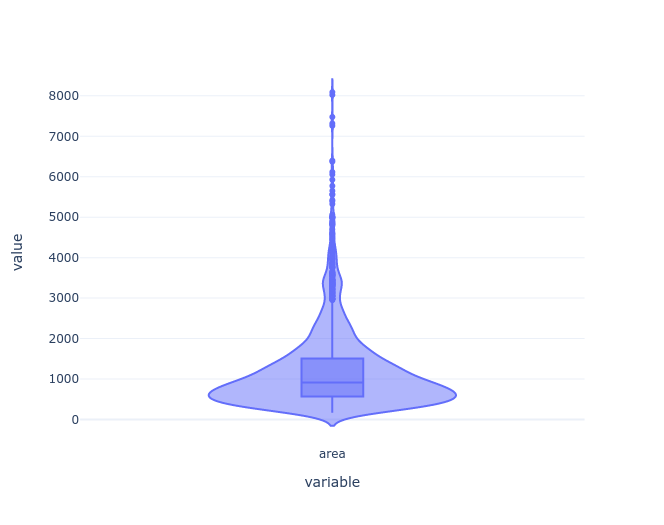
\includegraphics[width=0.5\textwidth]{figures/120_dataset/geometric_features area.png}
    }
    \subfloat[Feret diameter]{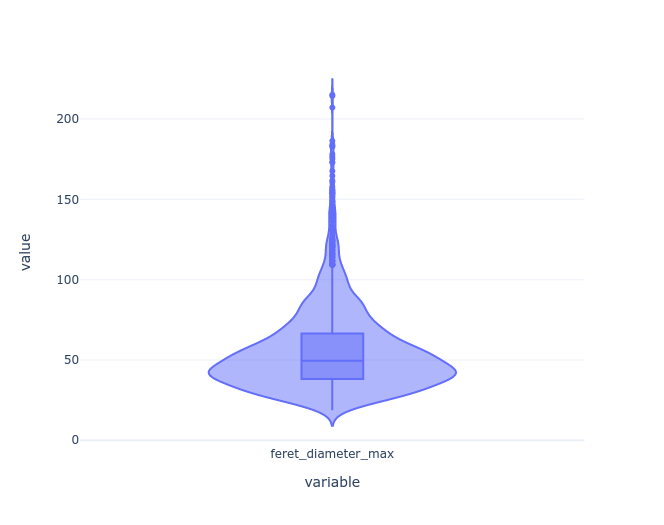
\includegraphics[width=0.5\textwidth]{figures/120_dataset/geometric_features feret.png}
    }
    \caption{\textbf{Geometrical features.} Distributions of the area (left) and maximum Feret diameter (right) across all annotated cells.}
    \label{fig:dataset:geom}
\end{figure}
After the initial exploration of the data characteristics at the pixel level, additional investigations can be devoted to discovering meaningful insights about images' macroscopic content.
Fluorescent Neuronal Cells pictures present a rich collection of neuronal cell instances differing in number, shape and size.

\Cref{fig:dataset:geom} shows the distributions of the most interesting geometrical features of the annotated objects.
On the left, the area distribution is shown. 
The bulk of the distribution presents cells with a surface within 358 and 1504 pixels.
On the right, the Feret diameter is reported \cite{merkus2009particle}. This measure is computed as the longest distance (in pixels) between points of a convex cell countour\footnote{obtained using skimage package version `0.18.1'}.
The distribution extends from a minimum of 18 to a maximum of 215 pixels, with the central 50\% concentrated in the range [38, 66].
In both cases, the distribution is left-skewed, with a slight prevalence of values lower than the median.
In fact, 90\% of objects are small and medium cells with prevalently regular circular shapes, having an area within [162, 2409] pixels and a Feret diameter between 18 and 88.
The remaining 10\% of the distribution stretches up to a maximum of 8092 and 215, respectively.
This effect is due to the contribution of more oversized or prolonged objects that cause a long, heavy tail.

\Cref{fig:dataset:counts_distrib} illustrates the distribution of the number of cells across the dataset.
In this case, the distribution presents multiple modes that can be summed up by the three major peaks, namely 6, 53 and 69
(\cref{fig:dataset:counts_hist}).
The empty spaces are a consequence of the fact that not all of the possible values were actually observed in the data.

By looking at the estimated density in the violin plot (\cref{fig:dataset:counts_violin}), it appears that the distribution can be interpreted as a mixture of two components.
%In particular, one can distinguish two peaks by looking at the estimated density in \cref{fig:dataset:counts_violin}.
The first is centered around 6 and is made of the images with lower counts, i.e. the ones depicting brain areas where the fluorophore did not reveal much activity of interest.
The second, instead, is a combination of the two higher peaks that represent active brain areas.
\begin{figure}
    \centering
    \subfloat[Histogram]{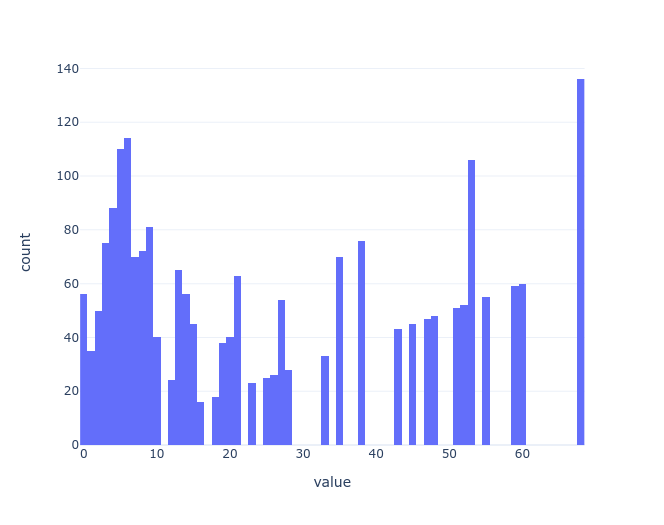
\includegraphics[width=0.5\textwidth]{figures/120_dataset/counts_histogram.png}
    \label{fig:dataset:counts_hist}
    }
    \subfloat[Violin plot]{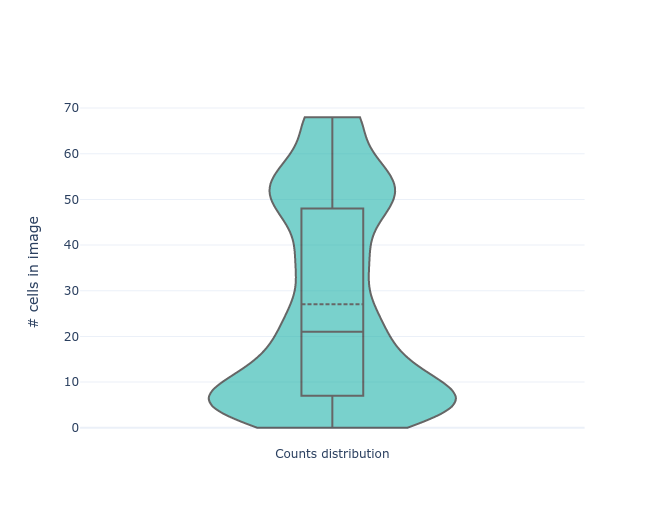
\includegraphics[width=0.5\textwidth]{figures/120_dataset/counts_violin.png}
    \label{fig:dataset:counts_violin}
    }
    \caption{\textbf{Counts distribution.} Distributions of the number of annotated cells across all images in the dataset.}
    \label{fig:dataset:counts_distrib}
\end{figure}